\documentclass{beamer}
\usepackage[english,russian]{babel}
\usepackage[utf8]{inputenc}
\usepackage{graphicx}
\usepackage{amssymb,amsmath}
\usepackage{float}
\usepackage{array}
\usepackage{ragged2e}
\usetheme[numbers]{Berlin}

\setbeamertemplate{caption}[numbered]
\pagestyle{plain} 
\setcounter{page}{0}


\begin{document}

\institute{МГУ имени М.В. Ломоносова, Москва, Россия}
\title{Отчет о выполнении II задания практикума}  
\author{Григорьева О. Константинова М. Козодой А.}
\date{ 2017\\Москва} 
\thispagestyle{empty}
\frame{\titlepage} 

\begin{frame}{Описание задания}
	После оглушительного успеха в освобождении Астапора, Миэрина и Юнкая от власти работорговцев Дейенерис Бурерожденная открыла себе доступ к Летнему морю, а следовательно -- путь в Вестерос.
	Для ведения войны с Семью Королевствами нужно оружие, а для оружия нужна сталь. Нет никаких сомнений в кузнечном искусстве Безупречных, однако поставщики стали не столь надежны.
	Два основных поставщика стали -- это Westeros Inc. и Harpy & Co. 
\end{frame}

\begin{frame}{Описание задания}
	На протяжении нескольких месяцев мы закупаем сталь у обеих компаний, и каждая из них предлагает ощутимую скидку при заключении эксклюзивного договора на поставку.
	Советник королевы Тирион Ланнистер знает о твоем умении принимать взвешенные рациональные решения и просит помощи в объективном решении вопроса о том, с какой из компаний следует заключить эксклюзивный договор на поставку стали.
	У Тириона есть записи о производстве мечей каждым из кузнецов-безупречных, а также данные о количестве сломанных мечей в каждый из месяцев ведения боевых действий.
\end{frame}


\begin{frame}{Выполнение задания. Часть 1.}
Необходимо провести разведывательный анализ данных с целью ответа на вопрос: "С каким из поставщиков стали следует заключить договор?" Работа ведется с  данными за прошедшие 7 месяцев из CSV-файла.	
Для этого считываем CSV-файл в матрицу и описываем необходимые нам для работы переменные.
Далее разделяем поток данных по двум компаниям, а для этого считаем два вектора prod{\_}sum{\_}co и prod{\_}sum{\_}inc соответсвующие двум компаниям - harpy&co и Westeros incorporate соовественно.
Каждый вектор содержит 6 значений, которые вычисляются по принципу:
1 месяц : производство за 1 месяц минус суммарный брак за 6 месяцев, и суммируется все по 50 кузнецам
2 месяц, соответственно, производство 2-ого минус суммарный брак, наблюдаемый за 5 месяцев и так далее.
\end{frame}

\begin{frame}{Выполнение задания. Часть 1.}
Диаграммы размахов, или "ящики с усами" (англ. box-whisker plots), получили свое название за характерный вид: точку или линию, соответствующую медианe, окружает прямоугольник ("ящик"), длина которого соответствует одному из показателей разброса или точности оценки генерального параметра. Дополнительно от этого прямоугольника отходят "усы", также соответствующие по длине одному из показателей разброса или точности. Графики этого типа очень популярны, поскольку позволяют дать очень полную статистическую характеристику анализируемой совокупности. Кроме того, диаграммы размаха можно использовать для визуальной экспресс-оценки разницы между двумя и более группами
\end{frame}

\begin{frame}{Выполнение задания. Часть 1.}
Далее строим описанный выше "ящики с усами"  для обеих компаний-производителей по таблице в которой первый столбец - это значения векторов, второй столбец соответсвующее название компании. 
Для этого используем функцию boxplot() и обозначаем диаграмму Harpy.co красным цветом, а Westeros.Inc - желтым.

\end{frame}

\begin{frame}{Выполнение задания. Часть 1.}	
	\begin{figure}[h]
		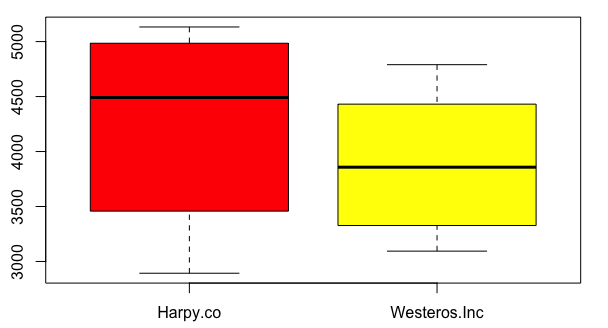
\includegraphics[width=100mm]{ysi}
		\caption{"Ящики с усами"}
		\label{ysi}
	\end{figure}
\end{frame}

\begin{frame}{Выполнение задания. Часть 2.}
Рассмотрим динамику поломок. 
Найдем количество  мечей, сделанных из стали компании Westeros.Inc и Harpy.co, сломавшихся в один из 6 месяцев, и попробуем определить, от чего оно зависит.
Оно может зависеть от: кузнеца, интенсивности боевых действий, качества стали и, возможно, еще каких-либо внешних параметров.
Методом пристального взгляда на таблицу мы устанавливаем, что кривые лучше искать отдельно для компаний.

\end{frame}

\begin{frame}{Выполнение задания. Часть 2.}
Проведя необходимые расчеты для стали компании Harpy.co, оказывается, что мечи из этой стали начинают ломаться только на 4 месяц использования. Причем это практически не зависит от кузнеца. Значения могут отличаться, но характер кривой для разных кузнецов сохраняется.
Аналогично проводим расчет и для стали Westeros.Inc. Мечи из этой стали ломаются примерно в равных количествах по месяцам. 
Эти результаты хорошо видно на рисунке.
\end{frame}

\begin{frame}{Выполнение задания. Часть 1.}	
	\begin{figure}[h]
		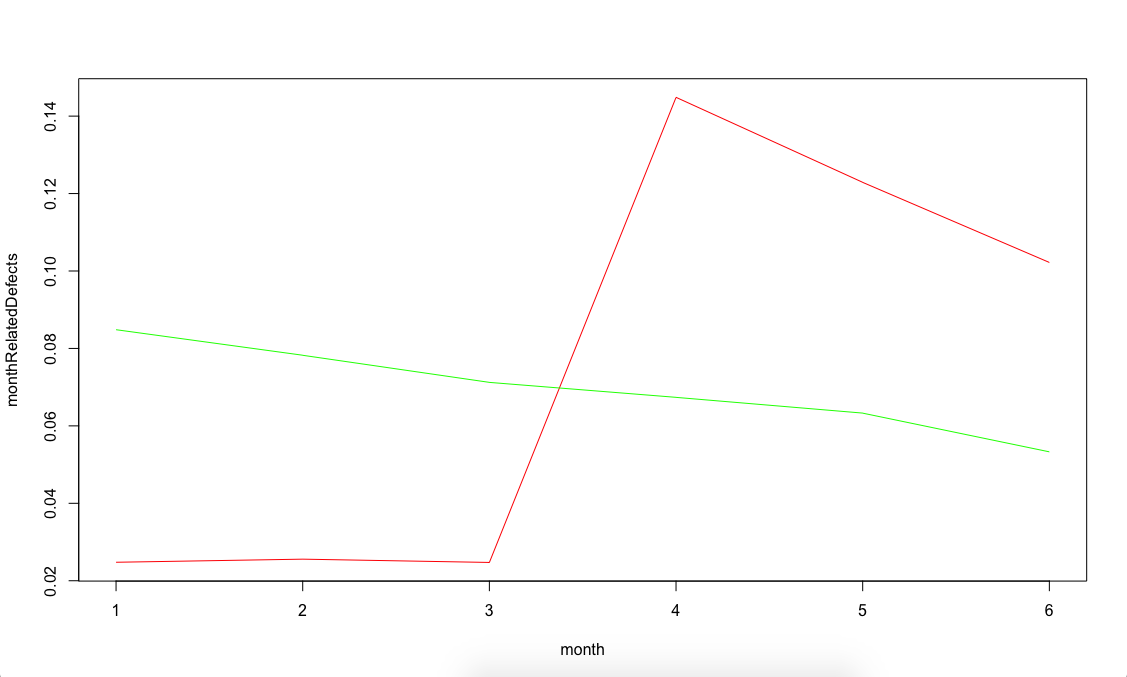
\includegraphics[width=100mm]{grafff}
		\caption{Графики ломкости мечей: red - Harpy.co, green -  Westeros.Inc.}
		\label{grafff}
	\end{figure}
\end{frame}

\begin{frame}{Выполнение задания. Часть 2.}
Небольшое убывание кривой по второй стали связано с тем, что общее количество целых мечей также убывает со временем.
Так как кривые сильно отличаются по компаниям, можем предположить, что интенсивность боевых действий не оказывает большого влияния (т.е. она была примерно постоянна за время наблюдения), как и внешние факторы.
\end{frame}



 

\begin{frame}{Анализ результатов. Часть 2.}
Как видно на рисунке 1, медиана Harpy.co выше медианы Westeros.Inc, пусть и разброс у первой компании больше. Высота медианы показывает, что показатели Harpy.co выше, а следовательно стоит выбрать именно эту компанию, основываясь на результатах первой части исследования. 
Из второй части исследования мы можем сделать такие выводы: 
Участь воина, у которого в бою сломался меч, не завидна, скорее всего, он быстро и бесславно погибнет. Таким образом, имеет смысл использовать сталь компании Harpy.co и выбрасывать мечи после приблизительно трех месяцев использования. Это позволит сохранить жизни воинов.

\end{frame}

\begin{frame}{Заключение. }
Обобщая результаты  исследования, получаем, что советнику Бурерожденной Тириону стоит посоветовать своей госпоже компанию Harpy.co.  
\begin{figure}[h]
		
\includegraphics[width=50mm]{tron}
		\caption{"Он будет нашим"}
		\label{tron}
	\end{figure}

\end{frame}

\begin{frame}{Задание выполняли}
	\begin{itemize}
		{\tiny \item Григорьева Олеся, студента 412 группы. Занималась разработкой подхода и написанием программы.
		\item Константинова Мария, студентка 412 группы. Разрабатывала подход к решению и писала отчет.
		\item Козодой Антон, студент 412 группы. Писал отчет и проводил анализ результатов.
				}
	\end{itemize}	
	

\end{frame}

\end{document}
